\chapter{Machine Learnings}
\label{ch:ml}

\par This chapter describes the Machine Learning (ML) / Artificial Intelligence (AI) system in the \vf which identifies triggers worthy of a closer look. First and foremost, the motivation is discussed in~\autoref{sec:coh}.
The ML model is introduced and described in~\autoref{sec:ml}. 
Lastly, the newly \emph{learnt} ML model is applied to the whole of \vfps~and results are examined in~\autoref{sec:ml_vfps}.

\section {Coherent analysis}
\label{sec:coh}

\par \vf operates on an \emph{incoherent} level. In all of the pipeline, only the power is considered.
There is no phase considered anywhere.
Hence the name, \emph{incoherent}.
This lack of phase greatly simplifies the pipeline design but comes at a cost.

\par For an array of $N$ antennas, co-addition in \emph{powers (incoherently)} (see~\autoref{ssub:needcoaddition}) only boosts the signal (or specifically, the signal-to-noise, \sn) by $\sqrt{N}$. 
A \emph{coherent} analysis would boost the \sn~by $N$. The reason being the phase information.

\par In addition to the \sn~boost, a \emph{coherent} analysis would also provide good localization capability.
Given a set of relative phases, one can translate to geometric delays and from there geometric path differences from asrophysical sources.
This ability is of great value since \frb s are known to be originating from outside the galaxy by which small angular variations could lead to astronomically large separated distances due to large radii.

\subsection{Coherent analysis with \vf}

\par The cost of doing a \emph{coherent} analysis real time is prohibitive. 
In order to be able to do \emph{coherent} analysis, voltage data has to be recorded. 
A second of raw voltage data consisting of two polarization measures about $250$ MB. 
A typical \vf compute node has $450$ GB of dedicated Solid State Disk (SSD). Meaning, a \vf compute can only have $1800$ s (or $30$ minutes) of raw voltage data before getting filled.
Given the extremely large volume of voltage data, it is impractical to record voltages all the time.
Hence, \vf performs searches \emph{incoherently} and triggers voltages for a coherent follow-up analysis.

\par It is also not practical to trigger voltages on all the triggers. It would be so as if voltages are recorded all the time since the trigger rates are high.
So only a subset of the triggers received are to be allowed to trigger voltages. 
Naturally, such a subset has to be selected on the basis of the signal's merit of being a real signal of astrophysical origin.
The question of how to decide what triggers to trigger on is the main goal of this chapter.

\section {Machine Learning}
\label{sec:ml}

\par The objective of the AI is to given a trigger, identify if a following \emph{coherent} analysis has to be initiated.
In an ideal situation, it would be desirous to have an AI solution which can identify all the true signals (i.e., the signals of interest).
However, training such an AI solution is extremely difficult.
The signals of interest are rare. Hence, any dataset produced would posses this assymmetric, which then would make training difficult.
Hence, this approach is abandoned. 
Succiently, the mission of the AI is to select those triggers which are worthy of a second closer look.

\par Any AI solution is only as good as the data used for training it. Keeping this in mind, the dataset is carefully created, which is discussed in~\autoref{ssub:dataset}. The model and training procedure used is described in~\autoref{ssub:mlmodel}.
The results from the training are showcased in~\autoref{ssub:training}.

\subsection{Dataset}

\label{ssub:dataset}

\par The problem at hand is a \emph{binary classification} problem. 
Every input is to be mapped to one of the two classes, either the \texttt{TRUE} class or the \texttt{FALSE} class.
Hence, the dataset used for training is so judiciously chosen such that it contains good representation of both the classes.

\par Triggers from known radio pulsars with \sn $\geq 7$ constitute a part of the \texttt{TRUE} class.
All the injected and received triggers also constitute the \texttt{TRUE} class.
RFI is manually selected using the creiterion described in~\autoref{ssub:rfim}.
The \dm{150} RFI is also selected and both form the \texttt{FALSE} class.
The actual breakdown of the cardinalities are given in~\autoref{tab:dataset}.

\par A separate dataset is chalked out and treated as \emph{unseen} dataset. This dataset will not be used in training or validation but will be used to see how the model performs on data which is not seen by it in any way.

% Please add the following required packages to your document preamble:
% \usepackage{booktabs}
\begin{table}[]
\label{tab:dataset}
	\begin{tabular}{@{}lll@{}}
		\toprule
		Dataset & Class & Number \\ \midrule
		VFPS & - & 818 848 \\ \midrule
		Injected & True & 8 480 \\
		Pulsars & True & 23 574 \\
		TRUE & - & 32 054 \\ \midrule
		RFI & False & 8 207 \\
		DM150 RFI & False & 20 660 \\ \midrule
		FALSE & - & 28 867 \\ \midrule
		Unseen & True & 1 716\\
		Unseen & False & 1 700\\ \bottomrule
	\end{tabular}
	\caption{The breakdown of \vfps dataset used for ML. See text.}
\end{table}

\subsection{Model and training}
\label{ssub:mlmodel}

\par A typical Convolutional Neural Network (CNN) is used here. The design of the CNN is depicted in~\autoref{fig:mlmodel}.
The non-linear activation used is the leaky-rectifier (\cite{lrelu}). To avoid overfitting dropouts (\cite{dropout,dropout2d}) are used after every layer.
To alleviate the covariant shift seen in deep layers, a batchnormalization layer is also added (\cite{batchnorm}) after certain layers.

\par The input of the CNN is two $32\times32$ image plane of de-dispersed filterbank and bowtie plane. 
The output is a two element vector showing the probabilities of the input belonging to both the classes.
A \dbson actually holds bowtie image of size $256\times256$ and de-dispersed filterbank of $64\times256$. 
These are reduced by block-means to same size of $32\times32$ and brought to $[0,1]$ by dividing by $255$.

\begin{figure}
	\label{fig:mlmodel}
	\centering
	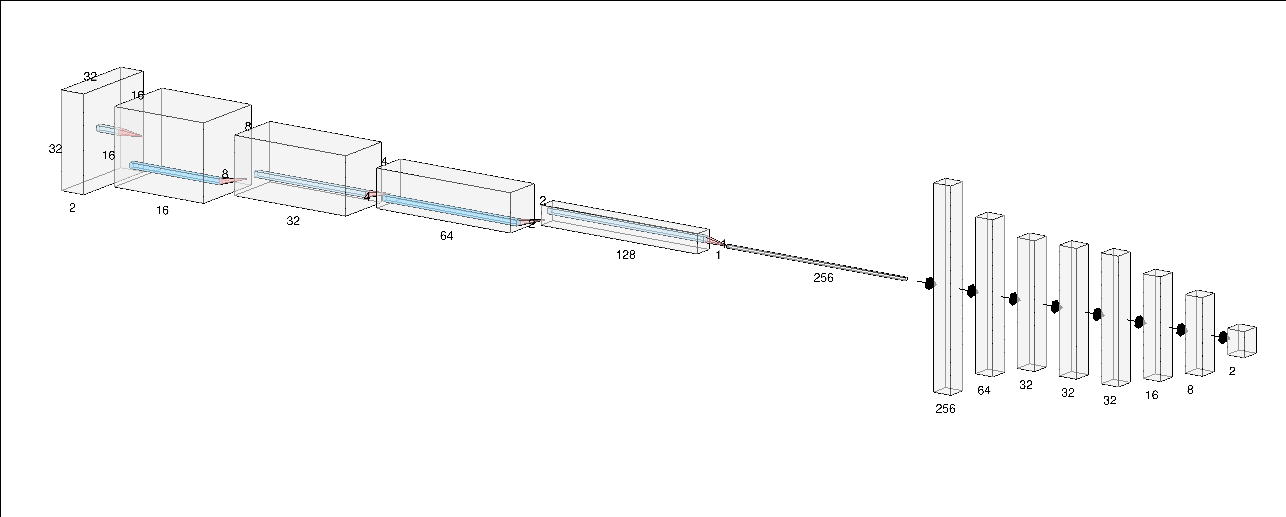
\includegraphics[width=0.8\textwidth, keepaspectratio]{zebel_model.png}
	\caption{CNN used in the AI. The numbers adjacent to the block represent the dimension of the block. Every block is followed bya dropout (~\cite{dropout2d,dropout}) and leaky-ReLU (~\cite{lrelu}). In addition, blocks with channels $32, 128$ also have a batchnormalization (\cite{batchnorm}). See text for model details. See \url{https://github.com/shiningsurya/trishul/tree/master/Python} for code.}
\end{figure}

\par Training was done in minibatches of 10. Two data augmentation transforms were employed:
\begin{enumerate}
	\item Frequency axis flip of de-dispersed filterbank.
	\item Time, \dm axes flip of bowtie plane.
\end{enumerate}
It is ensured that these two transformations don't cause the model to learn spurious features.
Adam optimizer (\cite{adam}) was used for optimizing. A step learning rate was employed. 
The loss function was CrossEntropyLoss since this is a classification problem.
The script which does the training is \url{https://github.com/shiningsurya/trishul/blob/master/Python/tscae_ig}.
Interested readers are encouraged to read the code.

\subsection{Training results}
\label{ssub:training}
\par The main training results are tabulated in~\autoref{tab:trainres}. 
The learning curves are plotted in~\autoref{fig:lcurves}.
The confusion matrices are tabulated in~\autoref{tab:traincfm}.

\par The metrics used to evaluate the performance are listed below. 
These metrics are computed from the confusion matrix.
A confusion matrix is a matrix showing how the AI has done the classification. A member of any class (\texttt{TRUE} or \texttt{FALSE}) can be classified as any other class by the AI.
This breakdown is tabulated in confusion matrix. A typical confusion matrix is shown in~\autoref{tab:cfm}.

\par A binary classification problem has two classes (\texttt{TRUE}, \texttt{FALSE}). Hence, a total of four possibilities can arise:
\begin{description}
	\item[True Positive (TP)] 
		When the AI classifies a \texttt{TRUE} class member correctly as a \texttt{TRUE} member.
	\item[False Positive (FP)] 
		When the AI classifies a \texttt{FALSE} class member incorrectly as a \texttt{TRUE} member. It is \emph{falsely} labeled as \emph{positive}.
	\item[True Negative (TN)] 
		When the AI classifies a \texttt{FALSE} class member correctly as a \texttt{FALSE} member.
	\item[False Negative (FN)] 
		When the AI classifies a \texttt{TRUE} class member incorrectly as a \texttt{FALSE} member. It is \emph{falsely} labeled as \emph{negative}.
\end{description}
Using these four definitions, one computes various point statistics to measure the perforamce.
% Please add the following required packages to your document preamble:
% \usepackage{booktabs}
\begin{table}[]
	\label{tab:cfm}
	\begin{tabular}{@{}lll@{}}
		\toprule
		 & TRUE & FALSE \\ \midrule
		TRUE & TP & FP \\
		FALSE & FN & TN \\ \bottomrule
	\end{tabular}
	\caption {A binary classification confusion matrix. Each row corresponds to what the AI thought the class would be. Each column is the ground truth. 
		If a candidate actually belongs to \texttt{FALSE} class (second column), if AI labels it as \texttt{TRUE}, it is treated as False Positive (FP). See text for more information.
	}
\end{table}

\begin{description}
	\item[Recall]
		shows the ability of AI to recover all the \texttt{TRUE} cases. Mathematically, it is written as $\frac{\rm TP}{\rm TP + FN}$.
	\item[Precision]
		shows the ability of AI to identify the \texttt{FALSE} cases. Mathematically, it is written as $\frac{\rm TP}{\rm TP + FP}$.
	\item[Accuracy]
		measures the gross performance of AI to classify both the cases. Mathematically, it is written as $\frac{\rm TP+TN}{\rm TN+FP+FN+TP}$.
	\item[False Positive Rate]
		measures the fraction of false positives over all the \texttt{FALSE} class. Mathematically, it is written as $\frac{\rm FP}{\rm FP+TN}$.
\end{description}

% Please add the following required packages to your document preamble:
% \usepackage{booktabs}
\begin{table}[]
	\label{tab:trainres}
	\begin{tabular}{@{}lllll@{}}
		\toprule
		Datasets & Recall & Precision & Accuracy & FPR \\ \midrule
		Training & 94.92 & 99.29 & 97.15 & 0.006 \\
		Validation & 94.60 & 99.24 & 97.01 & 0.006 \\
		Unseen & 73.54 & 99.14 & 86.38 & 0.006 \\ \bottomrule
	\end{tabular}
	\caption{Training results shown in various metrics computed. See text for metrics definitions.}
\end{table}

% Please add the following required packages to your document preamble:
% \usepackage{booktabs}
\begin{table}[]
	\label{tab:traincfm}
	\begin{tabular}{@{}ll|ll|ll@{}}
		\toprule
		\multicolumn{2}{l|}{Training} & \multicolumn{2}{l|}{Validation} & \multicolumn{2}{l}{Unseen} \\ \midrule
		22 933 & 160 & 5 735 & 39 & 1 689 & 11 \\
		1 125 & 21 017 & 299 & 5 236 & 454 & 1 262 \\ \bottomrule
	\end{tabular}
	\caption{Confusion matrices for different datasets. See text for more information.}
	\end{table}

\begin{figure}
	\label{fig:lcurves}
	\centering
	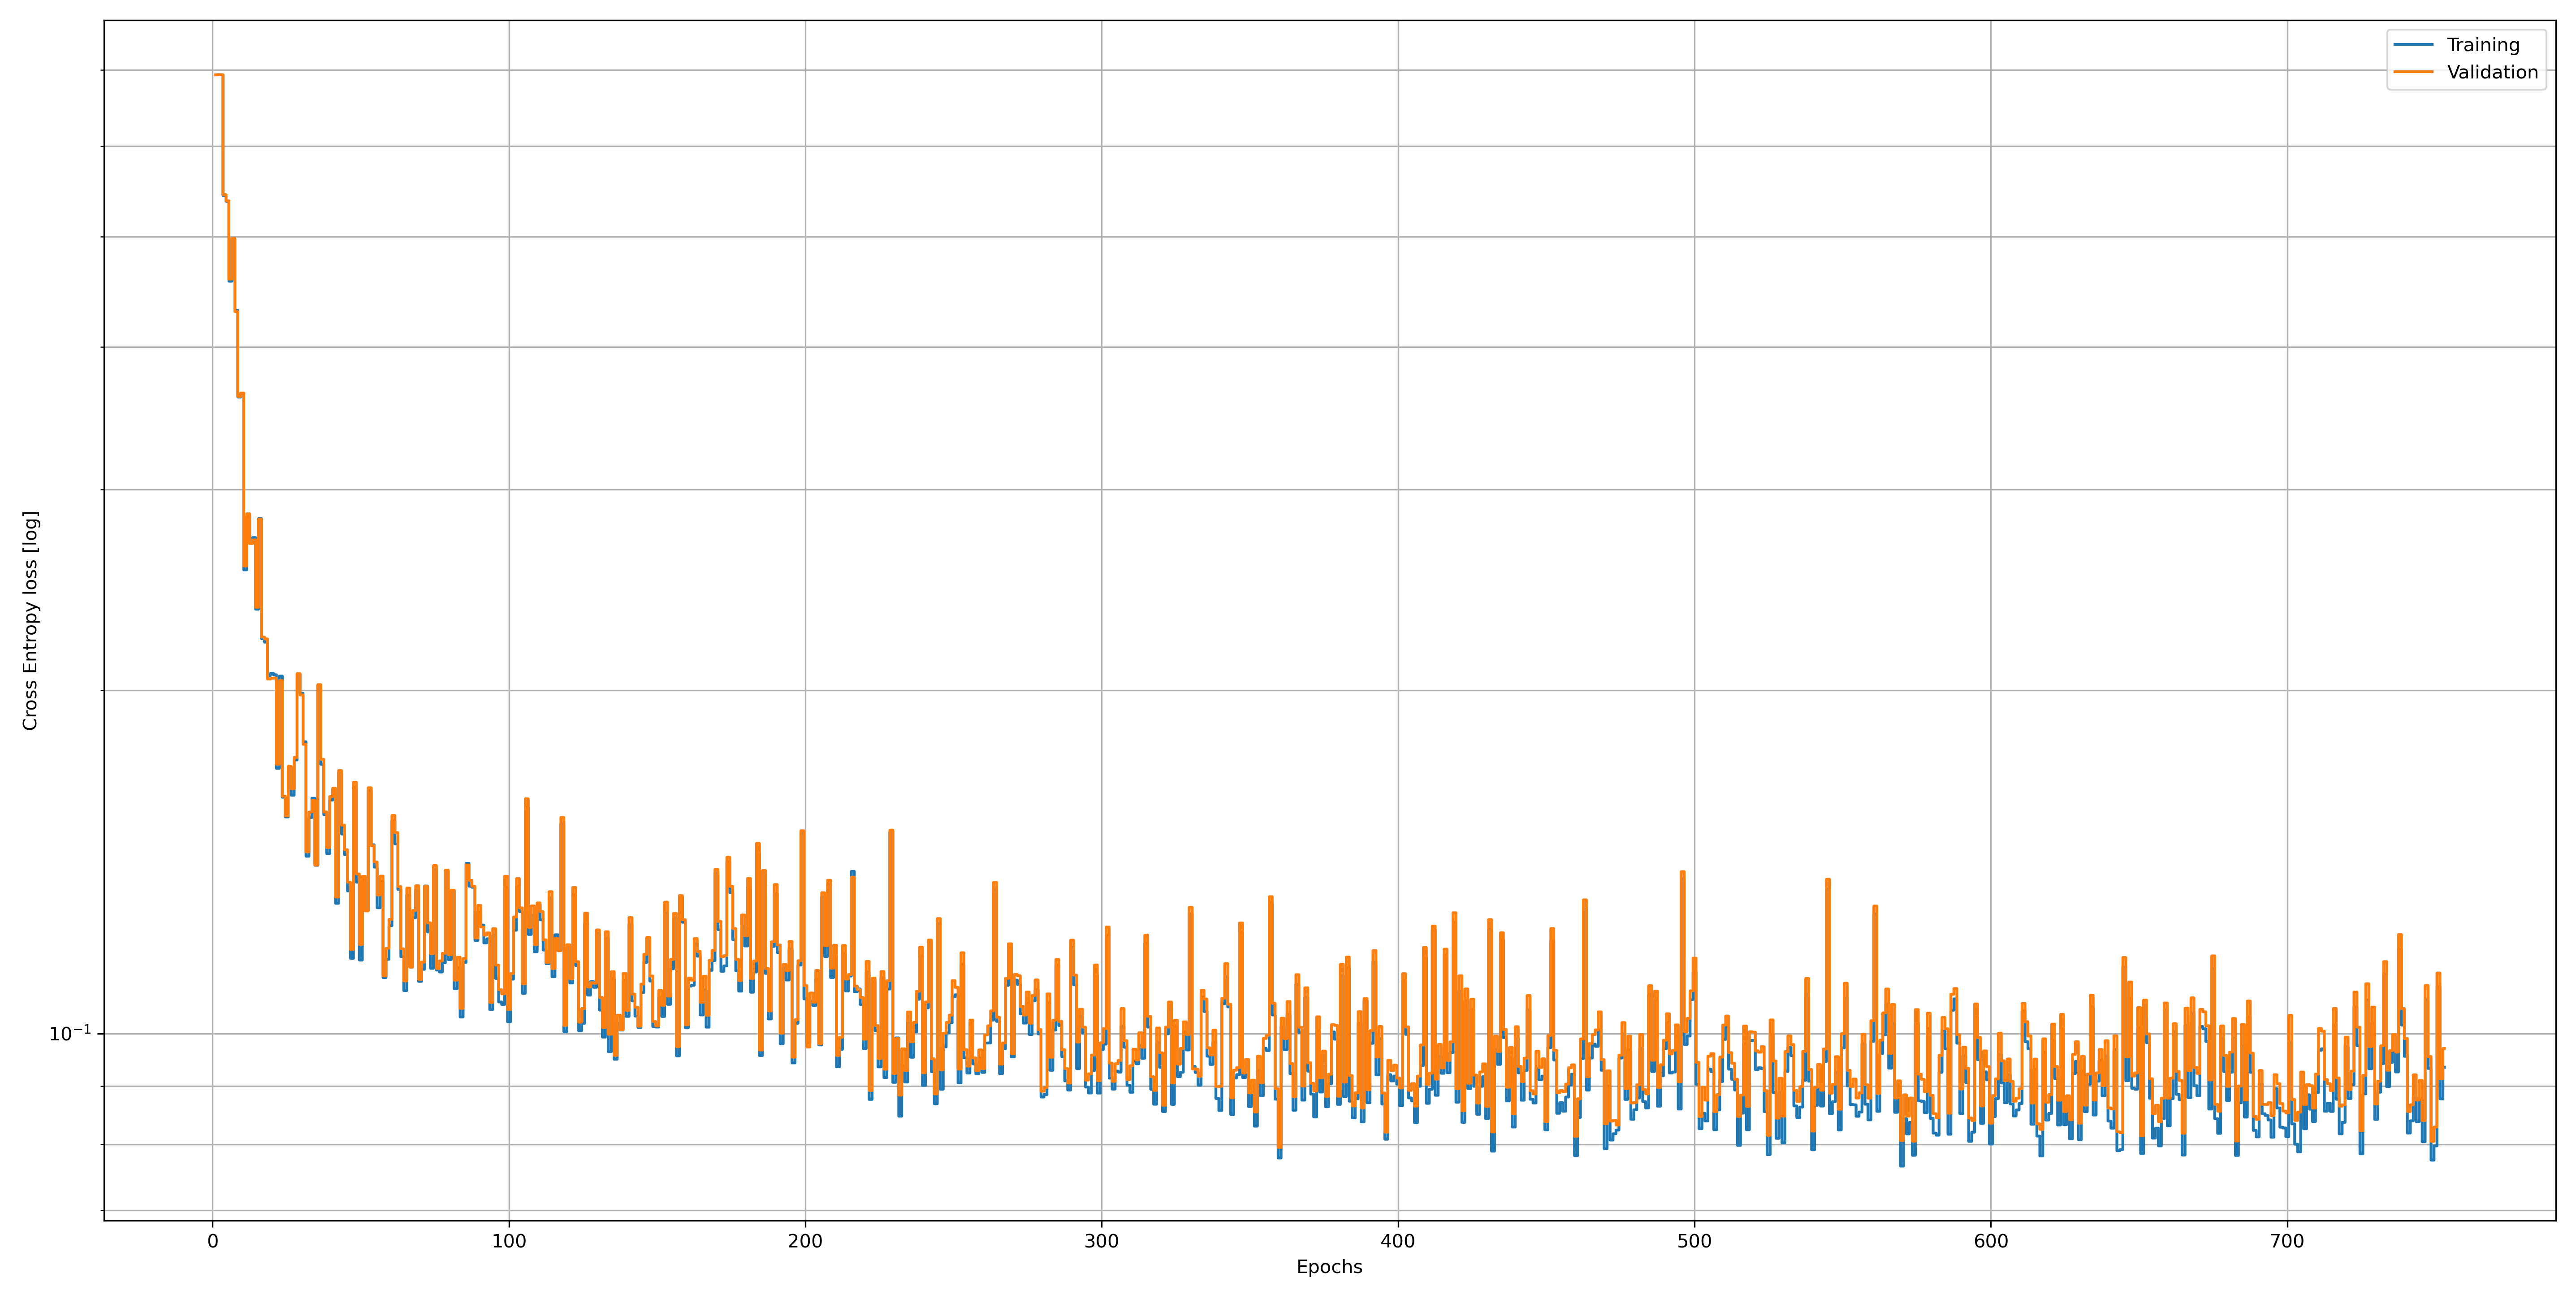
\includegraphics[width=0.8\textwidth, keepaspectratio]{learning_curves.png}
	\caption{Running for $753$ epochs. Model still can run for more epochs. GPU-based run done on Azure cloud took around a minute per epoch. This is a run lasting $\sim12^h$.}
\end{figure}

\section {VFPS ML inferences}
\label{sec:ml_vfps}

\par Having developed an ML solution trained on a very small subset, the AI is now run on the entire \vfps dataset.
Triggers selected by AI (henceforth just called selected triggers) are analyzed and reported.

\par The \dm~distribution of selected triggers is plotted in~\autoref{fig:inferdmdistro}. 
Naturally, the triggers from known pulsars are registered in bulk and are selected by the AI showing it's capability.
These bins are marked by solid red vertical lines. See~\autoref{tab:psrdetect} for the complete list of pulsars detected.

\begin{figure}
	\label{fig:inferdmdistro}
	\centering
	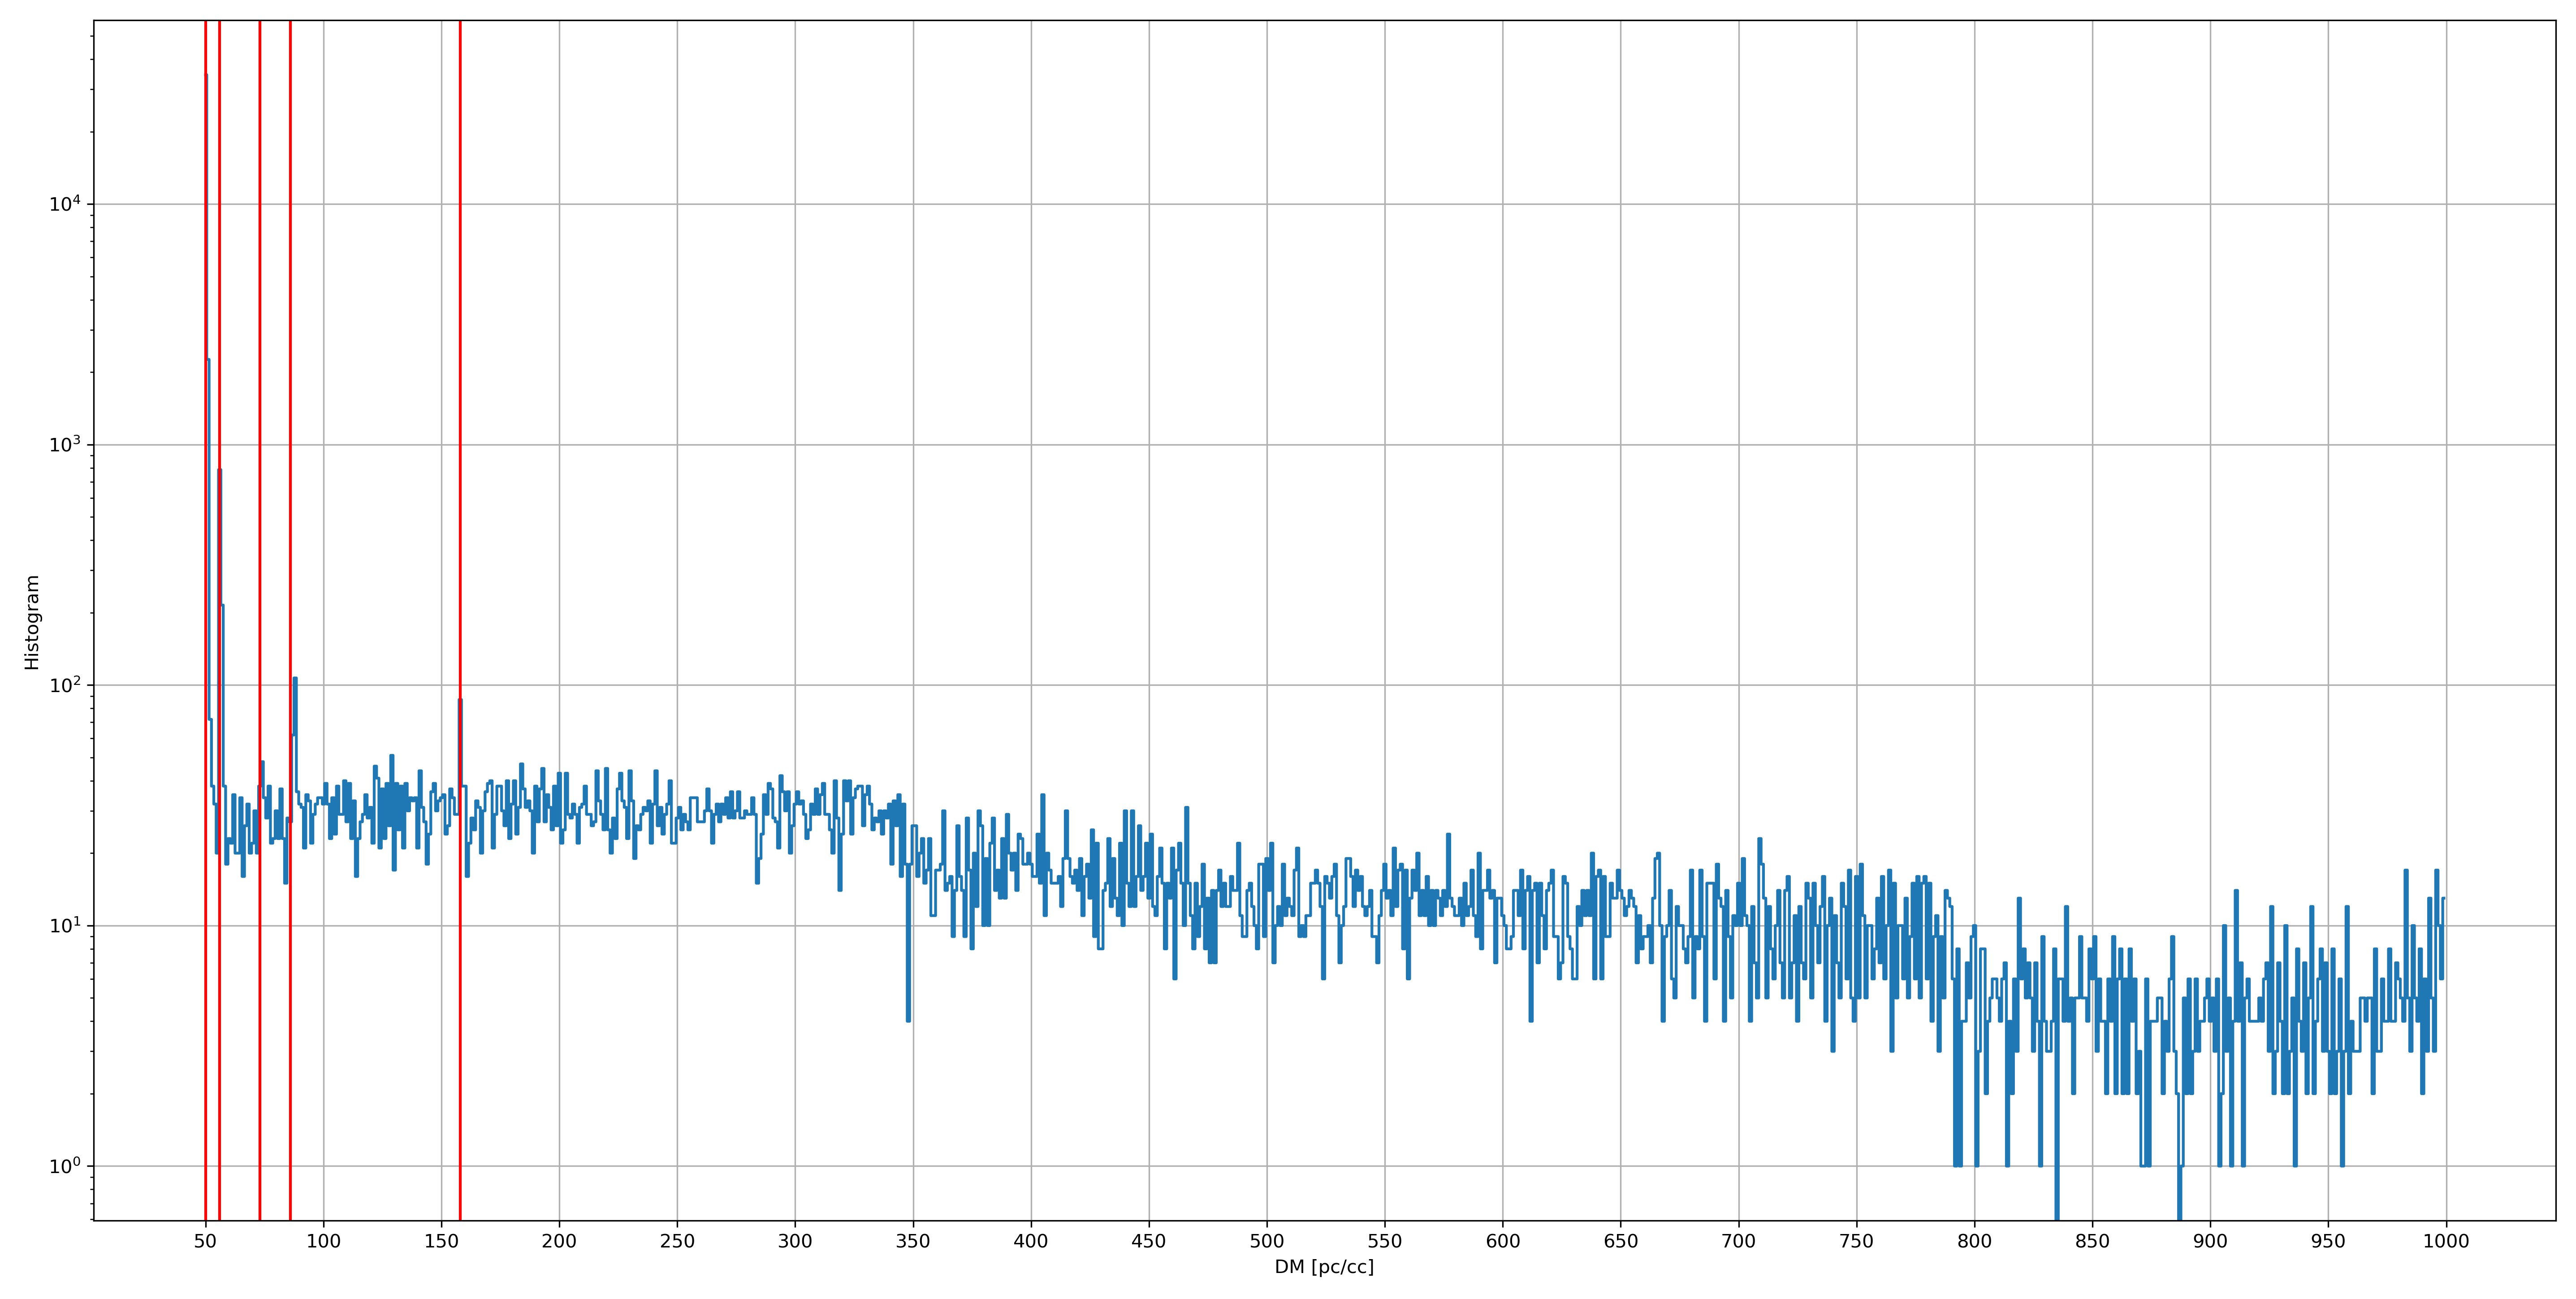
\includegraphics[width=0.8\textwidth, keepaspectratio]{dm_distro_vall_sf.png}
	\caption{\dm~distribution of AI selected triggers. Red vertical lines correspond to triggers from known pulsar (see~\autoref{tab:psrdetect}).}
\end{figure}

\par Since the pulsar triggers are already established, to make numbers managable, all known pulsar triggers are \dm-matched and dropped.
Performing a manual vetting yields one positive detection of trigger~\autoref{fig:isthisfrb}.
\texttt{PSRCAT}(\cite{psrcat}) doesn't have any pulsar around the \dm~near the field.
According to YMW16(\cite{ymw16}), the Galactic \dm~contribution is around $\sim 19$ implying an extremely high extra-galactic \dm~contribution.

\begin{figure}
	\label{fig:isthisfrb}
	\centering
	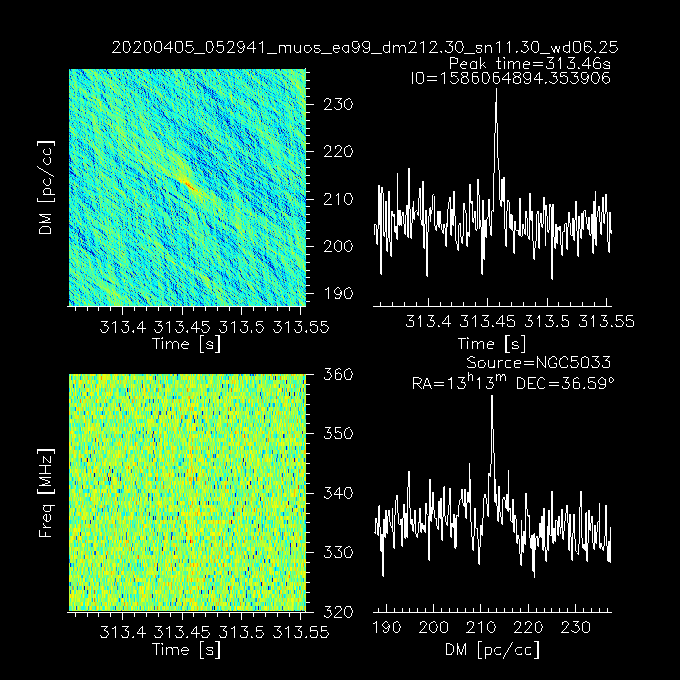
\includegraphics[width=0.8\textwidth, keepaspectratio]{isthisfrb.png}
	\caption{A possible \frb~candidate found after using AI developed in~\autoref{ch:ml} on \vfps~dataset}
\end{figure}

\section{Ending remarks}

\par The AI solution discussed here can be perfected. Moreover, the end goal of this AI is for it to be incorporated into the \vf pipeline for realtime vetting of the model.

